%%%%%%%%%%%%%%%%%%%%%%%%%%%%%%%%%%%%%%%%%
% Beamer Presentation
% LaTeX Template

\documentclass{beamer}


\mode<presentation> {

% Theme
\usetheme{metropolis}

%\setbeamertemplate{footline} % To remove the footer line in all slides uncomment this line
%\setbeamertemplate{footline}[page number] % To replace the footer line in all slides with a simple slide count uncomment this line

%\setbeamertemplate{navigation symbols}{} % To remove the navigation symbols from the bottom of all slides uncomment this line
}

\usepackage{graphicx} % Allows including images
\usepackage{booktabs} % Allows the use of \toprule, \midrule and \bottomrule in tables
\usepackage{cite}
\usepackage{natbib}
\usepackage{multirow}
\usepackage{rotating}



%----------------------------------------------------------------------------------------
%	TITLE PAGE
%----------------------------------------------------------------------------------------

\title[Short title]{Reproducible Research} % The short title appears at the bottom of every slide, the full title is only on the title page

\author{Marco Chiapello} % Your name
\institute[Center for Proteomics] % Your institution as it will appear on the bottom of every slide, may be shorthand to save space
{
Center for Proteomics\\
University of Cambridge \\ % Your institution for the title page
\medskip
\textit{mc983@cam.ac.uk} % Your email address
}
\date{\today} % Date, can be changed to a custom date

\begin{document}

\begin{frame}
\titlepage % Print the title page as the first slide
\end{frame}

\begin{frame}
\frametitle{Overview} % Table of contents slide, comment this block out to remove it
\tableofcontents % Throughout your presentation, if you choose to use \section{} and \subsection{} commands, these will automatically be printed on this slide as an overview of your presentation
\end{frame}

%----------------------------------------------------------------------------------------
%	PRESENTATION SLIDES
%----------------------------------------------------------------------------------------

%------------------------------------------------
\begin{frame}
\section{Introduction} % Sections can be created in order to organize your presentation into discrete blocks, all sections and subsections are automatically printed in the table of contents as an overview of the talk
\vspace{50px}
\begin{flushright}
\scriptsize {\bf Replication} is the ultimate standard by which scientific claims are judged\\ %\citep{Peng:2011et}
\scriptsize The fact that an analysis is reproducible does not guarantee the quality, correctness, or validity of the published results.
\end{flushright}
\end{frame}
%------------------------------------------------

%\subsection{Subsection Example} % A subsection can be created just before a set of slides with a common theme to further break down your presentation into chunks
\begin{frame}
\frametitle{What reproducible research is}
\begin{figure}
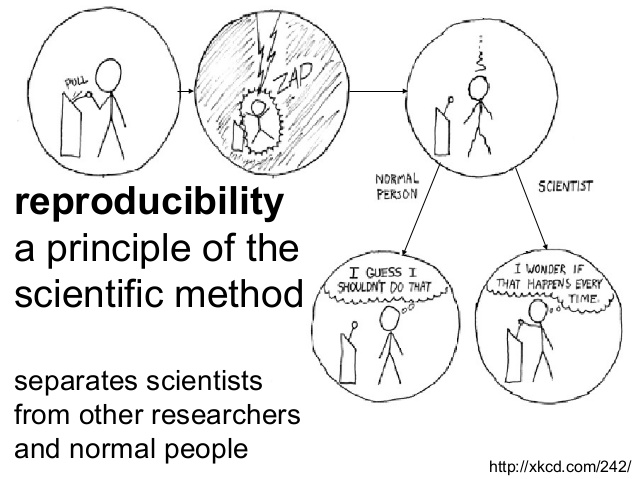
\includegraphics[scale=0.45]{figures/001.jpg}
\end{figure}
\end{frame}

%------------------------------------------------

\begin{frame}
\frametitle{What reproducible research is}
\begin{figure}
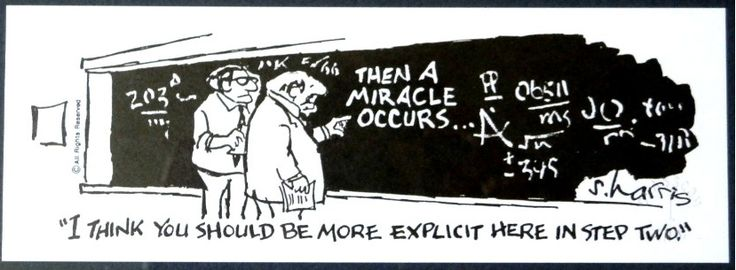
\includegraphics[scale=0.45]{figures/thenamiracleoccurs.jpg}
\end{figure}
\footnotesize 
\begin{itemize}
\item This is exactly how it seems when you try to figure out how authors got from a large and complex data set to a dense paper with lots of busy figures. \\Without access to the data and the analysis code, a miracle occurred. 
\item And  there should be {\sc no miracles in science.}%\cite{Markowetz:2016cs}
\end{itemize}
\end{frame}

%------------------------------------------------

\begin{frame}
\frametitle{What reproducible research is}
\Large\centering $DATA +  ANALYSIS \rightarrow RESULTS$\\
\rule{\textwidth}{0.05pt}\vspace{20px}

\centering{\sc\Large Reproducible vs Replicable}
\begin{table}[]
\centering
\begin{tabular}{cccc}
                                           &                                & \multicolumn{2}{c}{DATA}                          \\ \cline{3-4} 
                                           & \multicolumn{1}{c|}{}          & Same         & \multicolumn{1}{c|}{Different}     \\ \cline{2-4} 
\multicolumn{1}{c|}{\multirow{2}{*}{CODE}} & \multicolumn{1}{c|}{Same}      & Reproducible & \multicolumn{1}{c|}{Replicable}    \\
\multicolumn{1}{c|}{}                      & \multicolumn{1}{c|}{Different} & Robust       & \multicolumn{1}{c|}{Generalisable} \\ \cline{2-4} 
\end{tabular}
\end{table}

\end{frame}


%------------------------------------------------
\begin{frame}
Does reproducibility sound like extra work? It can be, particularly when one is first trying to do it, that is, to break one's own previous nonreproducible habits
\frametitle{Bullet Points}
\begin{itemize}
\item Lorem ipsum dolor sit amet, consectetur adipiscing elit
\item Aliquam blandit faucibus nisi, sit amet dapibus enim tempus eu
\item Nulla commodo, erat quis gravida posuere, elit lacus lobortis est, quis porttitor odio mauris at libero
\item Nam cursus est eget velit posuere pellentesque
\item Vestibulum faucibus velit a augue condimentum quis convallis nulla gravida
\end{itemize}
\end{frame}

%------------------------------------------------

\begin{frame}
\frametitle{Blocks of Highlighted Text}
\begin{block}{Block 1}
Lorem ipsum dolor sit amet, consectetur adipiscing elit. Integer lectus nisl, ultricies in feugiat rutrum, porttitor sit amet augue. Aliquam ut tortor mauris. Sed volutpat ante purus, quis accumsan dolor.
\end{block}

\begin{block}{Block 2}
Pellentesque sed tellus purus. Class aptent taciti sociosqu ad litora torquent per conubia nostra, per inceptos himenaeos. Vestibulum quis magna at risus dictum tempor eu vitae velit.
\end{block}

\begin{block}{Block 3}
Suspendisse tincidunt sagittis gravida. Curabitur condimentum, enim sed venenatis rutrum, ipsum neque consectetur orci, sed blandit justo nisi ac lacus.
\end{block}
\end{frame}

%------------------------------------------------

\begin{frame}
\frametitle{Multiple Columns}
\begin{columns}[c] % The "c" option specifies centered vertical alignment while the "t" option is used for top vertical alignment

\column{.45\textwidth} % Left column and width
\textbf{Heading}
\begin{enumerate}
\item Statement
\item Explanation
\item Example
\end{enumerate}

\column{.5\textwidth} % Right column and width
Lorem ipsum dolor sit amet, consectetur adipiscing elit. Integer lectus nisl, ultricies in feugiat rutrum, porttitor sit amet augue. Aliquam ut tortor mauris. Sed volutpat ante purus, quis accumsan dolor.

\end{columns}
\end{frame}

%------------------------------------------------
\section{Second Section}
%------------------------------------------------

\begin{frame}
\frametitle{Table}
\begin{table}
\begin{tabular}{l l l}
\toprule
\textbf{Treatments} & \textbf{Response 1} & \textbf{Response 2}\\
\midrule
Treatment 1 & 0.0003262 & 0.562 \\
Treatment 2 & 0.0015681 & 0.910 \\
Treatment 3 & 0.0009271 & 0.296 \\
\bottomrule
\end{tabular}
\caption{Table caption}
\end{table}
\end{frame}

%------------------------------------------------

\begin{frame}
\frametitle{Theorem}
\begin{theorem}[Mass--energy equivalence]
$E = mc^2$
\end{theorem}
\end{frame}

%------------------------------------------------

\begin{frame}[fragile] % Need to use the fragile option when verbatim is used in the slide
\frametitle{Verbatim}
\begin{example}[Theorem Slide Code]
\begin{verbatim}
\begin{frame}
\frametitle{Theorem}
\begin{theorem}[Mass--energy equivalence]
$E = mc^2$
\end{theorem}
\end{frame}\end{verbatim}
\end{example}
\end{frame}

%------------------------------------------------

\begin{frame}
\frametitle{Figure}
Uncomment the code on this slide to include your own image from the same directory as the template .TeX file.

\end{frame}

%------------------------------------------------

\begin{frame}[fragile] % Need to use the fragile option when verbatim is used in the slide
\frametitle{Citation}
An example of the \verb|\cite| command to cite within the presentation:\\

This statement requires citation \cite{p1}. 
\end{frame}

%------------------------------------------------

\begin{frame}
\frametitle{References}
\fontsize{6}{7.2}\selectfont
\bibliography{bib2}
\bibliographystyle{plainnat}
\end{frame}


%------------------------------------------------

\begin{frame}
\Huge{\centerline{The End}}
\end{frame}

%----------------------------------------------------------------------------------------

\end{document} 